%----------------------------------------------------------------------------
\chapter{次世代ピクセル検出器の量産}
\label{sec:singatapixel-devel}
%----------------------------------------------------------------------------
〜と同時に、HL-LHCアップグレードに向けた内部飛跡検出器の総入れ替えのため、次世代ピクセル検出器の開発が進められている。現在、ITkに搭載するモジュールについての


%----------------------------------------------------------------------------
\section{次世代ピクセル検出器の組み立て工程}
\label{sec:assemble}
%----------------------------------------------------------------------------
\begin{figure}[tbp]
  \centering
  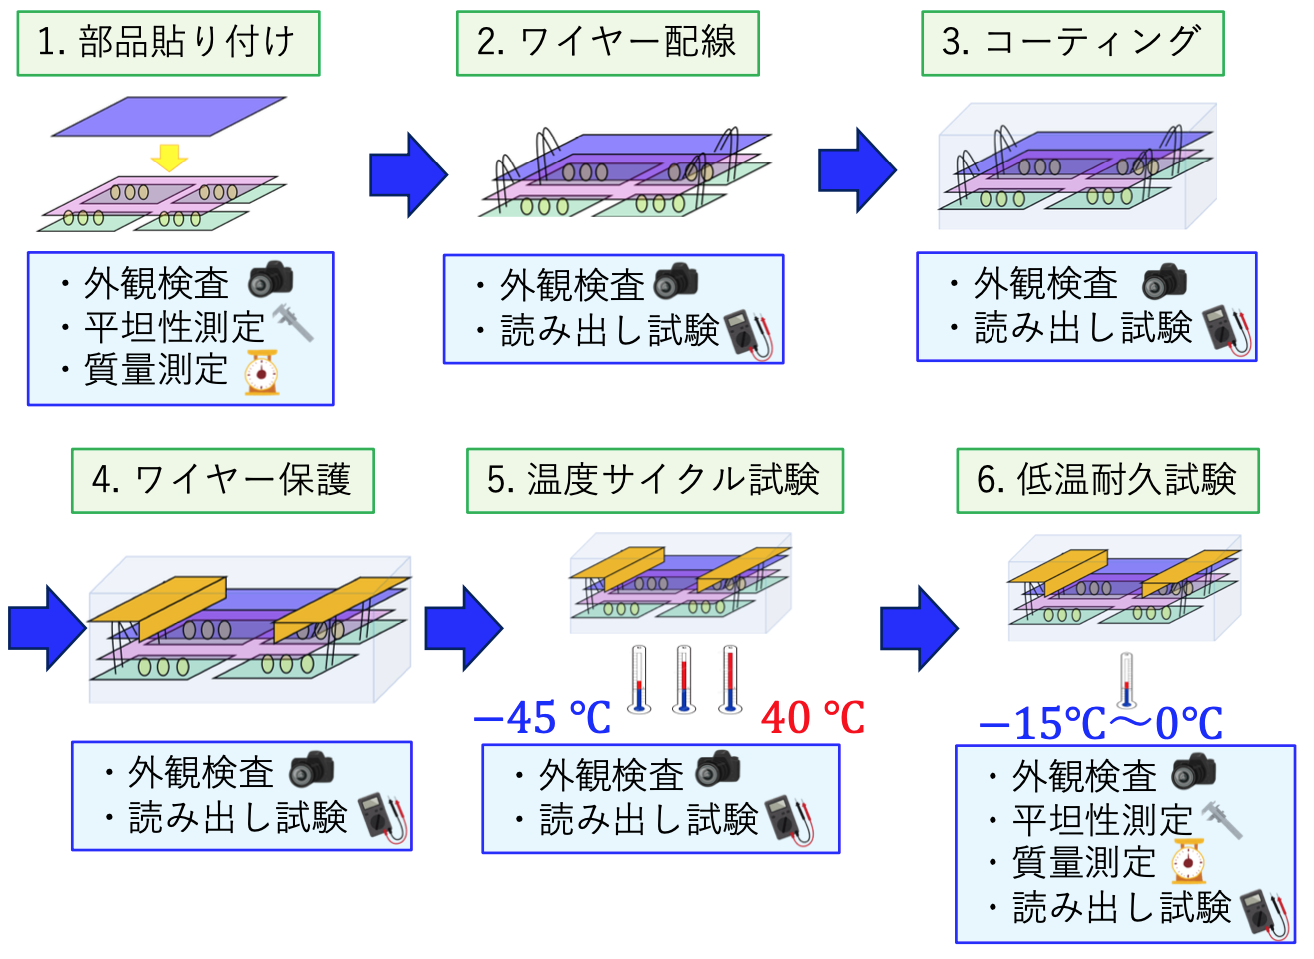
\includegraphics[height=7cm,keepaspectratio]{module_flow.png}
  \caption[ATLAS検出器]{ATLAS検出器の全体図 \cite{studyofID} }
  \label{fig:assemble}
\end{figure}


次世代ピクセル検出器の組み立て工程を\fref{fig:assemble}に示す。組み立て工程ではフレキシブル基板とベアモジュールの接着から始まり、ワイヤー配線、パリレン高分子によるコーティング、ワイヤー保護を行いピクセルモジュールが完成する。その後、温度サイクル試験および低温耐久試験において、運転時の温度環境においてモジュールが運用できるかの試験を行う。本節では、組み立て工程、およびモジュールの温度耐久についての試験についての説明を記す。

\begin{enumerate}
  \item 部品貼り付け
  \item ワイヤー配線
  \item コーティング
  \item ワイヤー保護
\end{enumerate}

\subsection{フレキシブル基板・ベアモジュールの接合}

\subsection{クーリングセルローディング}

\subsection{}

%----------------------------------------------------------------------------
\section{品質試験}
\label{sec:QC}
%----------------------------------------------------------------------------

\subsection{}

%----------------------------------------------------------------------------
\section{量産における試験結果管理}
\label{sec:}
%----------------------------------------------------------------------------



\newpage
